\section{Evaluation und Metriken}
\label{sec:eval_metrik}
Zur Beantwortung der Forschungsfragen werden die Algorithmen mit unterschiedlichen Hyperparameterkombinationen hinsichtlich ihrer Konvergenz und Spielstärke bewertet. Außerdem soll ermittelt werden, was laut den Agenten die optimale erste Aktion für das Symbol X ist.
Während der Trainings- und Evaluationsepsioden werden Daten gesammelt, auf Episoden-Ebene aggregiert und geloggt, sodass diese ausgewertet und geplottet werden können. 
Zum Plotten aller Liniendiagramme in dieser Arbeit wird die Python Bibliothek Matplotlib \cite{hunterMatplotlib2DGraphics2007} verwendet. 
Das dafür angefertigte Jupyter Notebook wird auf \href{http://github.com/JonasBingel/ThesisHSMZ-RLTicTacToe-Jupyter}{Github.com/JonasBingel} bereitgestellt.

Ein interessanter Aspekt beim Vergleich von RL-Algorithmen ist, wie schnell diese während des Trainings zur optimalen Policy konvergieren \cite[S. 33]{suttonReinforcementLearningIntroduction2018}. 
Als Konvergenzmetrik wird die Rate optimaler Aktionen, die vom Agent gewählt werden, genutzt.
Mit zunehmendem Lernen des Agenten sollte diese gegen 1 konvergieren. 
Während den Trainingsepisoden werden daher alle Aktionen des lernenden Agenten durch den Minimax-Algorithmus bewertet. 
Da sich die Rate zwischen den Episoden stark unterscheiden kann, werden die Werte der einzelnen Episoden kumuliert betrachtet. 
Zur Berechnung der Rate optimaler Aktionen gibt es zwei Möglichkeiten, da der Agent mit Wahrscheinlichkeit $\epsilon$ explorative Aktionen wählt. 
Einerseits \cref{eq:rate_inkl_exploration}, die die absolute Anzahl optimaler Aktionen inklusive explorativer Aktionen betrachtet.
Andererseits \cref{eq:rate_exkl_exploration}, die explorative Aktionen herausrechnet. 
Im Rahmen von Vorexperimenten wurde festgestellt, dass dies einen deutlichen Unterschied macht, wie \cref{fig:compare_rate} verdeutlicht.
Der Graph für \cref{eq:rate_exkl_exploration} nimmt aufgrund der Explorationswahrscheinlichkeit $\epsilon$ einmalig den Wert 1 oder 0 an.
Zu Beginn des Trainings gilt $\epsilon = 1$, sodass der Agent nur zufällige Aktionen wählt und folglich keine Rate für diese Episoden berechnet werden kann. 
Sinkt Epsilon mit fortschreitender Episodenanzahl, kann der Agent selbst eine Aktion wählen. 
Da der Agent zu Beginn jedoch nur einzelne Aktionen wählt, nimmt die Rate optimaler Aktionen kurzfristig Extremwerte an.

Die Formel in \cref{eq:rate_inkl_exploration} hat den Vorteil, dass der aktuelle Zustand des Agenten in dieser Episode erfasst wird. 
Jedoch bietet \cref{eq:rate_exkl_exploration} einen besseren Vergleichsmaßstab, da diese den Agenten als fertige Strategie bewertet, die während der Evaluation getestet wird. 
Für die Auswertung der Agenten wird in dieser Arbeit \cref{eq:rate_exkl_exploration} verwendet. 

\begin{equation}\label{eq:rate_inkl_exploration}\equationentry{Rate optimaler Aktionen \inkl Exploration}
   \text{Rate}_{\text{mit Exploration}} = \frac{\text{Anzahl optimaler Aktionen}}{\text{Anzahl Aktionen des Agenten}}
\end{equation}

\begin{equation}\label{eq:rate_exkl_exploration}\equationentry{Rate optimaler Aktionen \exkl Exploration}
   \text{Rate}_{\text{ohne Exploration}} = \frac{\text{Anzahl optimaler Aktionen ohne Exploration}}{\text{Anzahl Aktionen des Agenten} - \text{Anzahl explorativer Aktionen}}
\end{equation}

\begin{figure}[h]
    \centering
    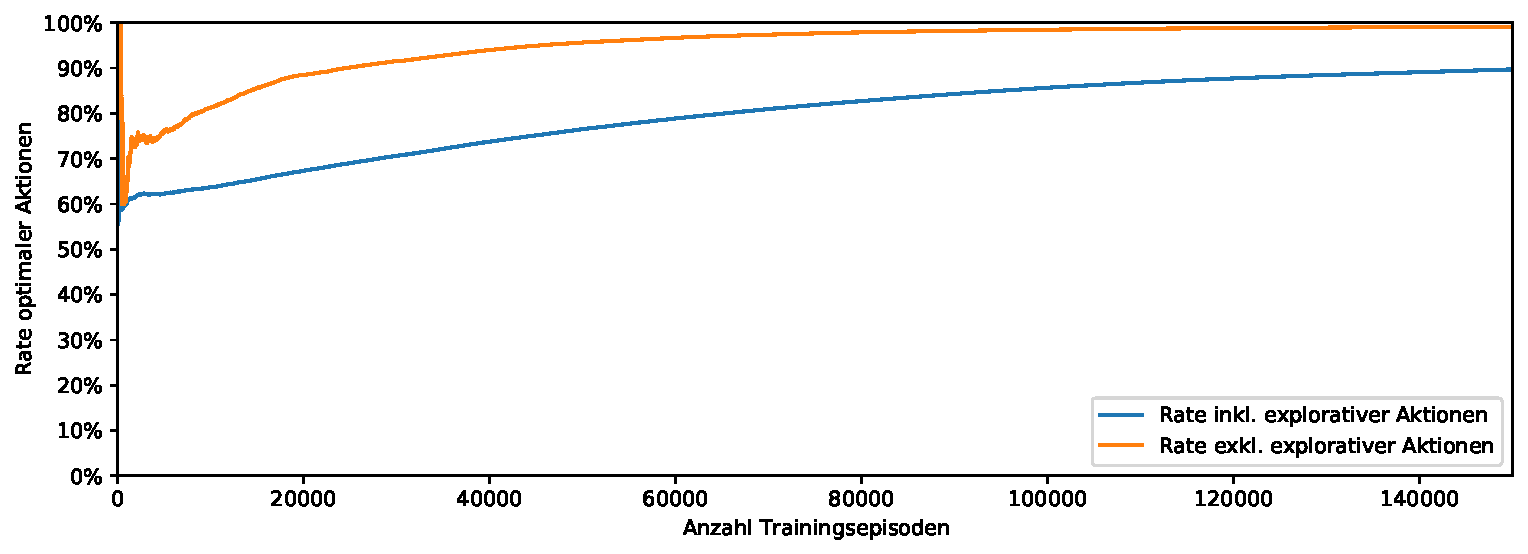
\includegraphics[scale=0.5]{convergence/convergence_compare_rate_X.pdf}
    \caption{Vergleich der Raten optimaler Aktionen}
    \label{fig:compare_rate}
\end{figure}

Um die Spielstärke der trainierten Agenten zu messen, spielt der Agent jeweils 10.000 Evaluationsspiele für beide Symbole X und O. 
Die Hyperparameter $\alpha, \epsilon$ des Agenten werden auf 0 gesetzt, damit die greedy Policy genutzt wird und kein Lernen erfolgt. 
Zum einen spielt der Agent gegen den Minimax-Algorithmus. 
Sollten mehrere Aktionen optimal sein, wählt Minimax aus dieser Menge zufällig aus, sodass unterschiedliche Zustände evaluiert werden. 
Zum anderen spielt der Agent gegen einen Spieler mit Zufallstrategie Random, damit seine Spielstärke gegen einen nicht optimalen Gegner ermittelt werden kann. 
Aufgrund von Vorexperimenten wurde festgelegt, dass fünf Agenten trainiert und das arithmetische Mittel von deren Evaluationsspielen genutzt wird, um eine bessere Vergleichbarkeit der trainierten Agenten zu ermöglichen.

Die Spielstärke kann quantifiziert werden, wenn die Spielergebnisse mit der in \cref{sec:TDL_TTT} beschriebenen Rewardfunktion bewertet werden.
In den insgesamt 20.000 Spielen gegen Minimax, kann bestenfalls ein Gesamtreward von 0 erzielt werden, da Minimax optimal spielt und das Spiel somit nur in einer Niederlage oder einem Unentschieden enden kann. 
In \cref{tab:reward_depth_penalty} wurde gezeigt, dass X frühestmöglich nach fünf und O nach sechs Zügen gewinnen kann. 
Unter der unrealistischen Annahme, dass ein Spieler jedes Spiel gegen Random in möglichst wenigen Aktionen gewinnt, beträgt der bestmögliche Reward somit 9.000, wie \cref{eq:spielstaerke_intervall} zeigt. 
Der schlechteste theoretische Wert ist -18.000 und beschreibt das Szenario, in dem jedes Spiel gegen Minimax und Random in einer schnellstmöglichen Niederlage endet.
Das Intervall der Spielstärke beträgt somit $[-18.000;9.000]$

\begin{equation}
\label{eq:spielstaerke_intervall}
\equationentry{Berechnung des Intervalls der Spielstärke}
\begin{split}
    \text{beste Spielstärke} = 20.000 \cdot 0 + 10.000 \cdot 0,5 + 10.000 \cdot 0,4 = 9.000 \\
    \text{schlechteste Spielstärke} = 20.000 \cdot -0,5 + 20.000 \cdot -0,4 = -18.000
\end{split}
\end{equation}